\documentclass{article}

% Language setting
% Replace `english' with e.g. `spanish' to change the document language
\usepackage[german]{babel}

% Set page size and margins
% Replace `letterpaper' with `a4paper' for UK/EU standard size
\usepackage[a4paper]{geometry}

% Useful packages
\usepackage{amsmath}
\usepackage{graphicx}
\usepackage[colorlinks=true, allcolors=blue]{hyperref}
\usepackage{float}
\usepackage{multicol}
\usepackage{xcolor}

\setlength{\columnseprule}{0.5pt}
\def\columnseprulecolor{\color{blue}}


\title{Wirtschaft für Ingenieure}
\author{Asha Schwegler}

\begin{document}
\maketitle

\section{Grundprinzipien der Betriebswirtschaft}

\paragraph{Ökonomisches Prinzip:}
Spannungsverhältnis zwischen Unbegrenzte Bedürfnisse\\
und knappe Ressourcen.

\subsection{Gütereinteilung}
\paragraph{Güter werden aufgeteilt in:}

\begin{itemize}
\item Freie Güter
\item Wirtschaftliche Güter
\end{itemize}

\begin{figure}[H]
\centering
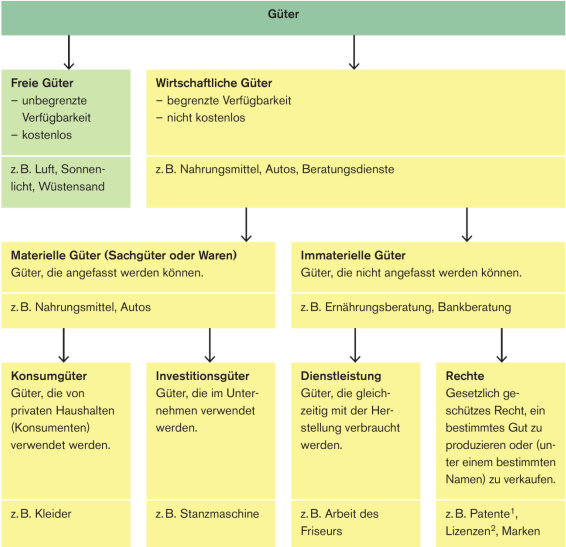
\includegraphics[width=0.3\textwidth]{Resources/Image/Guetereinteilung.png}
\caption{\label{fig:Guetereinteilung}Guetereinteilung.}
\end{figure}


\subsection{Markt}
Der Markt besteht aus Zusammenwirkung von Nachfrage und Angebot. \\
\subparagraph{Nachfrage:} Entsteht aus Bedarf, der wiederum aus Bedürfnisse entsteht.
\subparagraph{Angebot:} 
Entsteht aus der Herstellung


\subsection{Dreifache Unternehmensverantwortung}
\paragraph{Balance Akt zwischen:} 

\begin{itemize}
\item Gesamterhalt (Planet)
\item Selbsterhalt (Profit)
\item Miterhalt (People)
\end{itemize}

\begin{figure}[H]
\centering
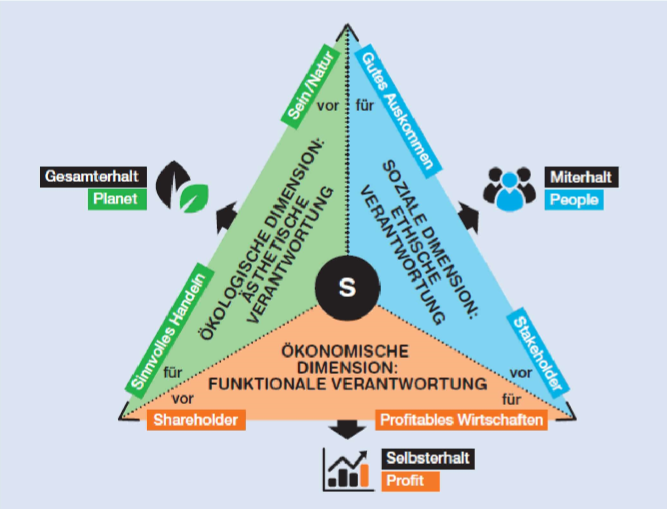
\includegraphics[width=0.3\textwidth]{Resources/Image/Dreifache Unternehmungsveratntwortung.png}
\caption{\label{fig:DreifacheUnternehmungsverantwortung}DreifacheUnternehmungsverantwortung.}
\end{figure}


\subsection{St. Galler Managementmodell}
\begin{figure}[H]
\centering
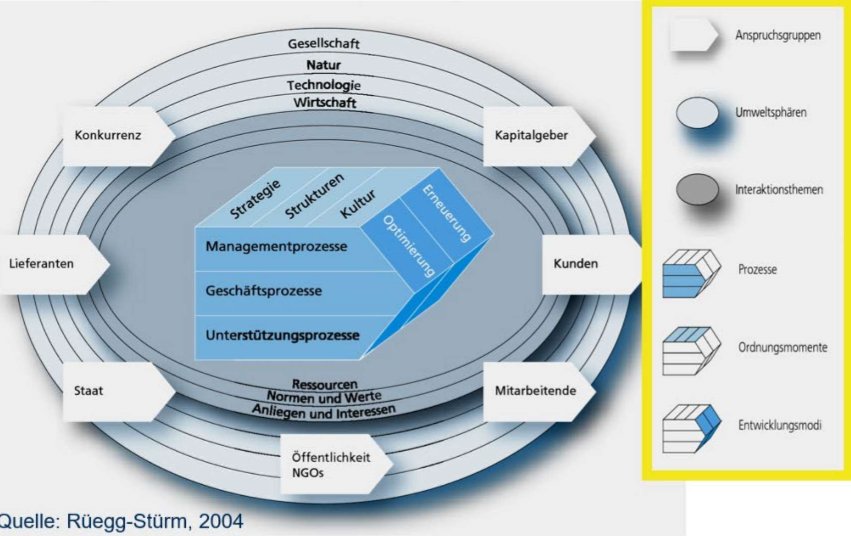
\includegraphics[width=0.3\textwidth]{Resources/Image/SGMM.png}
\caption{\label{fig:SGMM}SGMM.}
\end{figure}


\subsubsection{Umweltsphären}

\begin{tabular}{|l|l|}
\hline 
\rule[-1ex]{0pt}{2.5ex} \textbf{Umweltsphären} & \textbf{Beobachtungsbereiche} \\ 
\hline 
\rule[-1ex]{0pt}{2.5ex} Ökonomische Umwelt & Entwicklung Wirtschaft, Arbeitsmarkt, Teuerung, Wirtschaftsbeziehungen zum Ausland etc. \\ 
\hline 
\rule[-1ex]{0pt}{2.5ex} Technologische Umwelt & Produktionsverfahren, Materialien, Transport- und Kommunikationsmittel etc. \\ 
\hline 
\rule[-1ex]{0pt}{2.5ex} Soziale Umwelt & Politische und gesellschaftliche Trends, Wohlbefinden der einzelnen Menschen etc. \\ 
\hline 
\rule[-1ex]{0pt}{2.5ex} Ökologische Umwelt & Rohstoffe, Energie, Klima, Abfälle, etc. \\ 
\hline 
\end{tabular} 


\subsubsection{Anspruchsgruppen / Stakeholder}
\begin{enumerate}
\item Sind von der Tätitigkeit der Unternehmen betroffen. 
\item Haben Erwartungen und Ansprüche.
\end{enumerate}
 

\subparagraph{Machtausübung Primär:}
\begin{itemize}
\item faktische
\item vertragliche
\item gesetzliche
\item oder normative Grundlagen
\end{itemize}


\subparagraph{Sanktionsgrundlage Sekundär:}
\begin{itemize}
\item gesellschaftspolitische
\item witschaftsethische Konventionen
\end{itemize}

\begin{figure}[H]
\centering
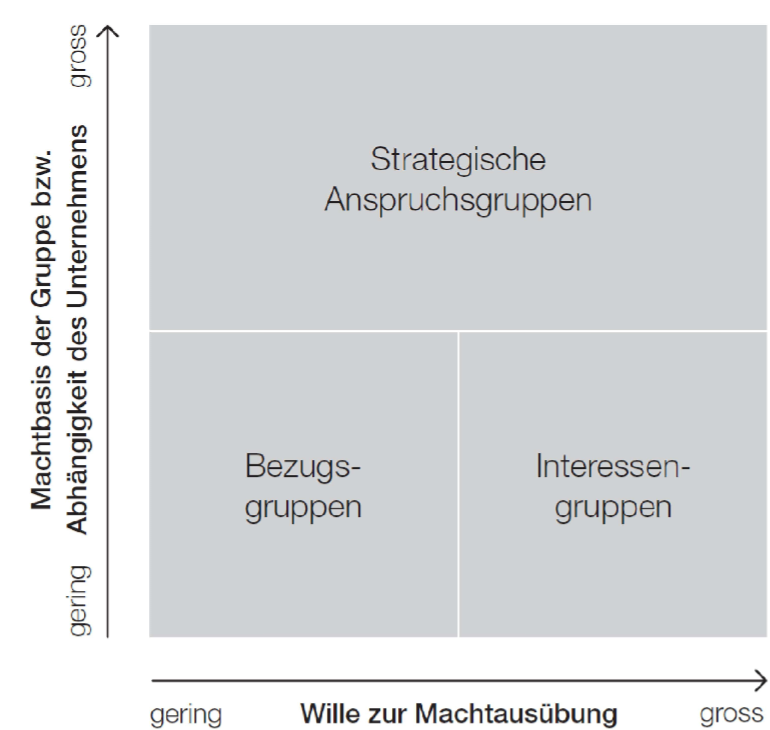
\includegraphics[width=0.3\textwidth]{Resources/Image/MachtausuebungStakeholder.png}
\caption{\label{fig:MachtausuebungStakeholder}MachtausuebungStakeholder.}
\end{figure}

\subsubsection{Interaktionsthemen}

\paragraph{Interaktionsthemenanalyse:}
\begin{enumerate}
\item Bestimmte Anspruchsgruppe
\item Anliegen und Interessen aufzeigen
\item Vorliegende Normen und Werte prüfen
\end{enumerate}

\paragraph{Ressourcen:}
\begin{enumerate}
\item Arbeit, Boden, Kapital, Wissen
\item Marke, Reputation, Image, Vertrauen
\end{enumerate}


\paragraph{Vorgehen:}

\subparagraph{1. Sachverhalt:}
\begin{itemize}
\item Welche Ressource des Unternehmens ist betroffen
\item In Welche Umweltsphäre spielt sich Sachverhalt ab
\end{itemize}

\subparagraph{2. Welche Anspruchsgruppe:}
\begin{itemize}
\item Anliegen / Ziele
\item Interessen
\item Normen (Gesetze und Regeln)
\item Werte
\end{itemize}

\subparagraph{3. Aus Unternehmenssicht:}
\begin{itemize}
\item Gefahren
\item Reaktionsmöglichkeiten
\end{itemize}

\begin{figure}[H]
\centering
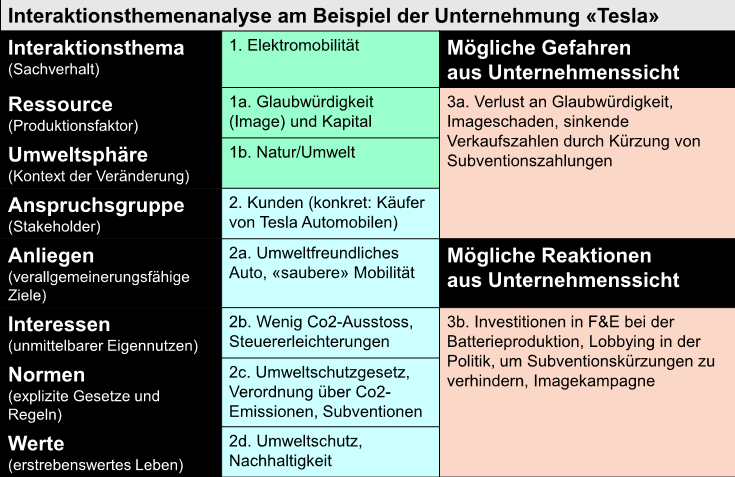
\includegraphics[width=0.3\textwidth]{Resources/Image/Interaktionsthemenanalyse.png}
\caption{\label{fig:Interaktionsthemenanalyse}Interaktionsthemenanalyse.}
\end{figure}

\pagebreak
\section{Strategie}
\title\textbf{Einordnung:\\}
\begin{figure}[H]
\centering
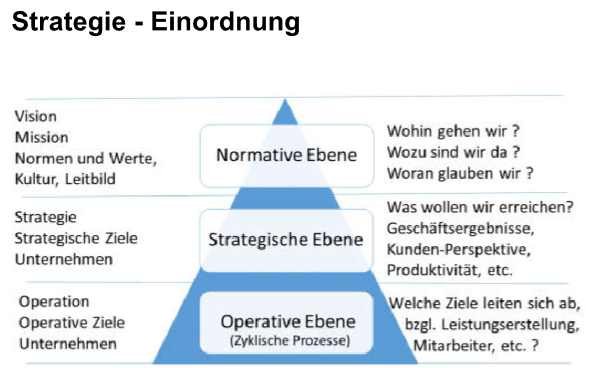
\includegraphics[width=0.3\textwidth]{Resources/Image/StrategieEinordnung.png}
\caption{\label{fig:StrategieEinordnung}StrategieEinordnung.}
\end{figure}

\title\textbf{Für Management-Entscheide:\\}
\begin{figure}[H]
\centering
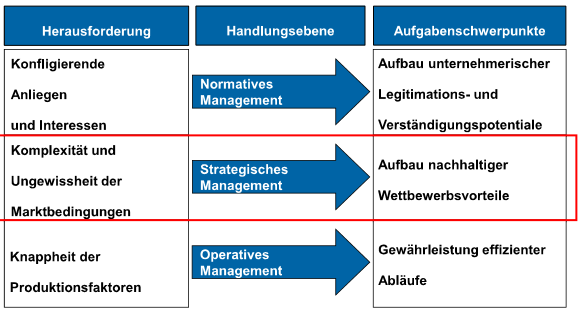
\includegraphics[width=0.3\textwidth]{Resources/Image/ManagementEntscheide.png}
\caption{\label{fig:ManagementEntscheide}ManagementEntscheide.}
\end{figure}


\subsection{Strategiefindungsprozess}
\paragraph{In vier Schritten:}
\begin{enumerate}
\item Strategische Analyse
\item Strategische Planung
\item Strategische Umsetzung
\item Strategische Messung
\end{enumerate}
\pagebreak
\subsection{Die strategische Analyse}
\subparagraph{Drei Modellen:}
\begin{itemize}
\item SWOT-Analyse
\item PESTEL-Analyse
\item 5-Forces Modell von Porter
\end{itemize}

\subparagraph{Faktoren, die Analyse beeinflussen\\}
\begin{figure}[H]
\centering
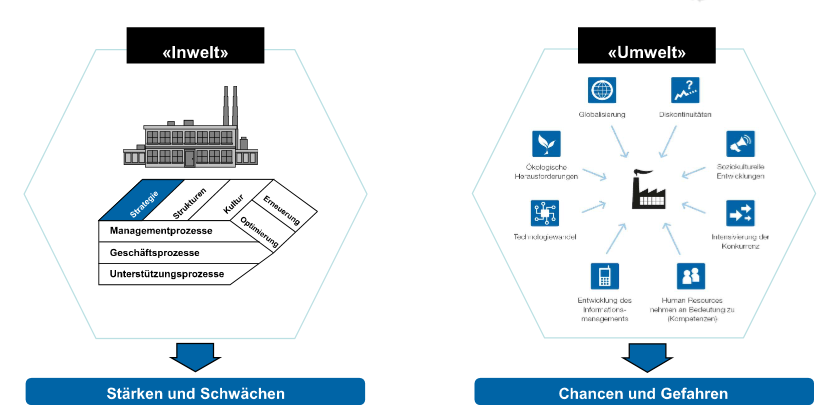
\includegraphics[width=0.3\textwidth]{Resources/Image/FaktorenEinfluss.png}
\caption{\label{fig:FaktorenEinfluss}FaktorenEinfluss.}
\end{figure}

\subsubsection{SWOT-Analyse:}
\begin{figure}[H]
\centering
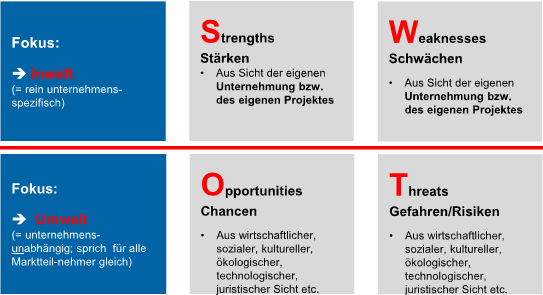
\includegraphics[width=0.3\textwidth]{Resources/Image/SwotAnalyse.png}
\caption{\label{fig:SwotAnalyse}SwotAnalyse.}
\end{figure}

\subparagraph{Kern-Kompetenzen:}

Kompetenz als Wettbewerbsvorteil
\begin{itemize}
\item Wertvoll
\item Selten
\item Nicht oder schwer imitierbar
\item Nicht substituierbar
\end{itemize}


\paragraph{Unternehmensanalyse Beispiel Easyjet \\ \\}

\begin{tabular}{|l|c|}
\hline
\rule[-1ex]{0pt}{2.5ex} 
\textbf{Strenghts} & \textbf{Weaknesses} \\ 
\hline 
\rule[-1ex]{0pt}{2.5ex}
Moderne Flugzeuge mit tiefen Betriebskosten & Keine Interkontinentalflüge \\ 
\hline 
\rule[-1ex]{0pt}{2.5ex}
Ersten Fluggesellschaften,Internetplattform zum Buchen & Gewisse (teure)Flughäfen  nicht Streckennetz \\ 
\hline
\rule[-1ex]{0pt}{2.5ex} 
Einheitliches Angebot (Bloss Ecenomy Class etc) &  \\ 
\hline
\rule[-1ex]{0pt}{2.5ex}
\end{tabular} \\ \\


\begin{tabular}{|l|l|}
\hline 
\rule[-1ex]{0pt}{2.5ex}
\textbf{Opportunities} & \textbf{Threats} \\ 
\hline 
\rule[-1ex]{0pt}{2.5ex} Wetter(Schlecht in CH zu Gut Ausland) & Covid-19 Reisebeschränkungen \\ 
\hline 
\rule[-1ex]{0pt}{2.5ex} Trend Wochenend Städtereisen & Verteuerung Treibstoffkosten \\ 
\hline 
\rule[-1ex]{0pt}{2.5ex} Grössere Flugzeuge & Höhere Flughafentaxen \\ 
\hline 
\rule[-1ex]{0pt}{2.5ex} Steigender Wohlstand & Verlängerung Nachtflugsperre europ.Flughafen \\ 
\hline 
\rule[-1ex]{0pt}{2.5ex}  & Neue Billig-Airlines \\ 
\hline 
\end{tabular} 
\\
\\

\title\textbf{Die vier abgeleiteten Grundstrategieansätze: \\}
\begin{figure}[H]
\centering
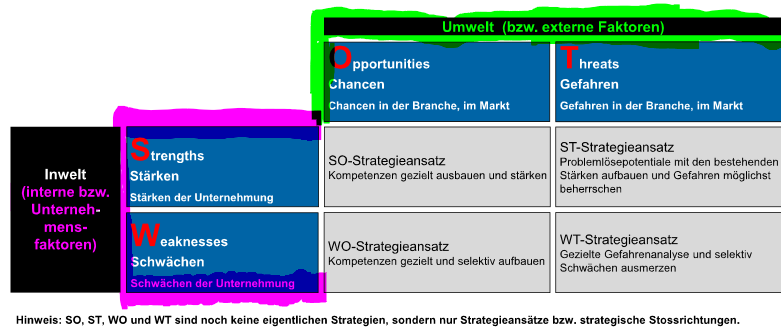
\includegraphics[width=0.3\textwidth]{Resources/Image/GrundstrategieAnsaetze.png}
\caption{\label{fig:GrundstrategieAnsaetze}GrundstrategieAnsaetze.}
\end{figure}


\subsubsection{PESTEL-Analyse}

Untersucht den Einfluss der sechs \textbf{externen} Umweltfaktoren \\
\begin{figure}[H]
\centering
\includegraphics[width=0.3\textwidth]{Resources/Image/Pestelanalyse.png}
\caption{\label{fig:Pestelanalyse}Pestelanalyse.}
\end{figure}




\subsubsection{5 Kräfte Modell von Porter}

Untersucht den Markt. \\

\begin{figure}[H]
\centering
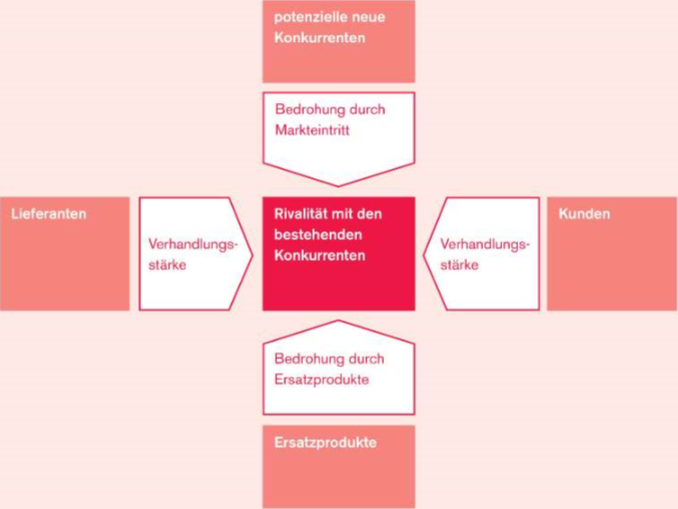
\includegraphics[width=0.3\textwidth]{Resources/Image/Porteranalyse.png}
\caption{\label{fig:Porteranalyse}Porteranalyse.}
\end{figure}


\begin{figure}[H]
\centering
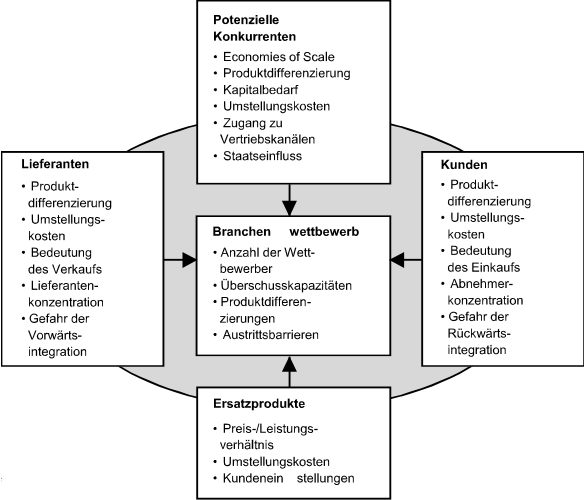
\includegraphics[width=0.3\textwidth]{Resources/Image/ZFPorter.png}
\caption{\label{fig:ZFPorter}ZFPorter.}
\end{figure}

\title\textbf{Branchenanalyse EasyJet\\}

\begin{figure}[H]
\centering
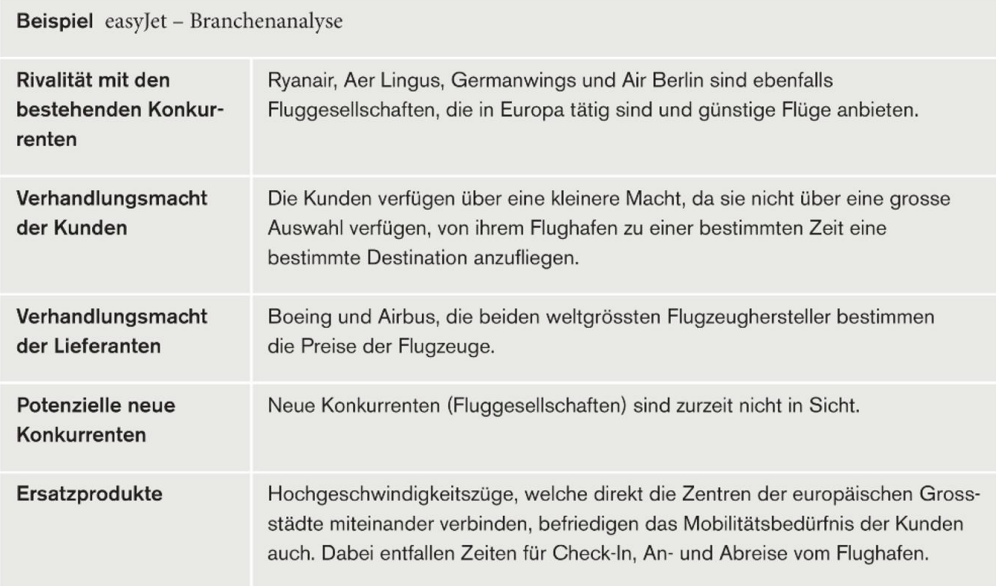
\includegraphics[width=0.3\textwidth]{Resources/Image/Branchenanalyse.png}
\caption{\label{fig:Branchenanalyse}Branchenanalyse.}
\end{figure}


\title\textbf{Entwicklung einer Strategie \\}
\begin{figure}[H]
\centering
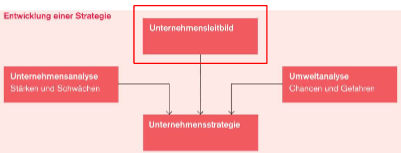
\includegraphics[width=0.3\textwidth]{Resources/Image/Strategieentwicklung.png}
\caption{\label{fig:Strategieentwicklung}Strategieentwicklung.}
\end{figure}


\title\textbf{Unternehmensleitbild \\}
\begin{figure}[H]
\centering
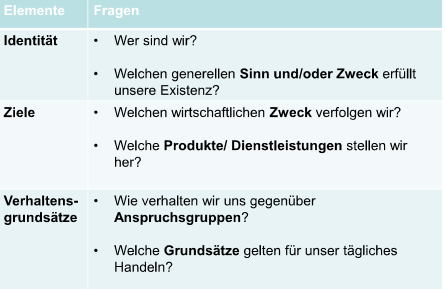
\includegraphics[width=0.3\textwidth]{Resources/Image/Unternehmensleitbild.png}
\caption{\label{fig:Unternehmensleitbild}Unternehmensleitbild.}
\end{figure}
\pagebreak
\title\textbf{Unternehmensstrategie\\}
\begin{figure}[H]
\centering
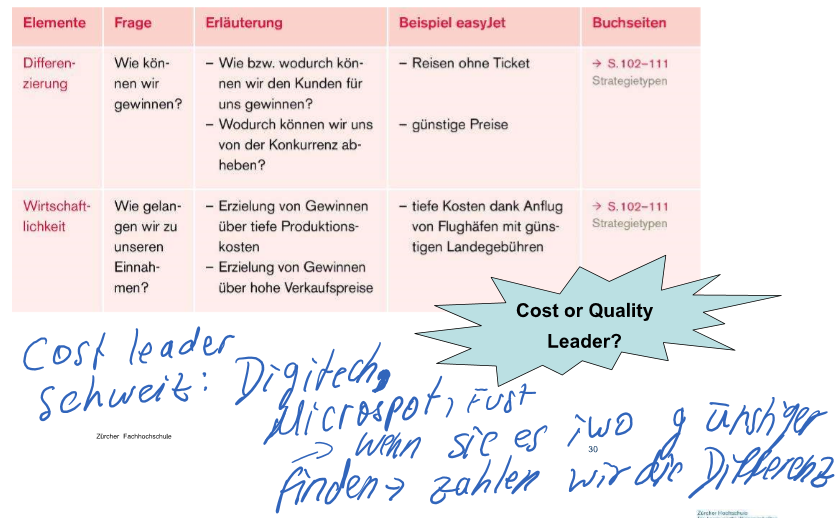
\includegraphics[width=0.3\textwidth]{Resources/Image/Unternehmensstrategie.png}
\caption{\label{fig:Unernehmungsstrategie}Unternehmensstrategie.}
\end{figure}



\subsection{Die Strategische Planung}

Hier geht es um die \textbf{Strategieformulierung und -auswahl \\}

\paragraph{zwei Modelle: \\}
\begin{enumerate}
\item 4-Branchenwettbewerbsstrategien nach Porter
\item 4-Produkt-Markt-Strategien nach Ansoff
\end{enumerate}


\begin{Large}
\title\textbf{4-Branchenwettbewerbsstrategien nach Porte \\}
\end{Large}

\begin{figure}[H]
\centering
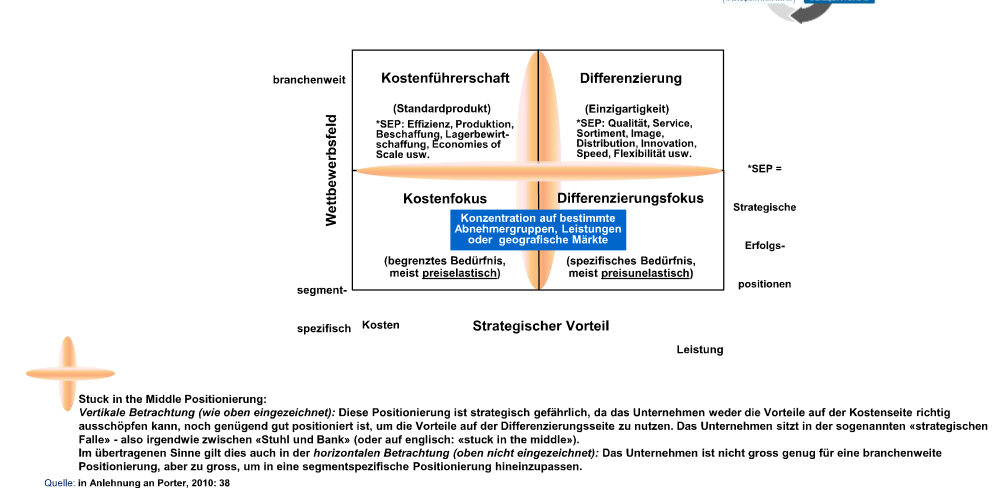
\includegraphics[width=0.3\textwidth]{Resources/Image/PorterWettbewerbstrategie.png}
\caption{\label{fig:PorterWettbewerbstrategie}PorterWettbewerbstrategie.}
\end{figure}



\begin{Large}
\title\textbf{4-Produkt-Markt-Strategien nach Ansoff \\}
\end{Large}

\begin{figure}[H]
\centering
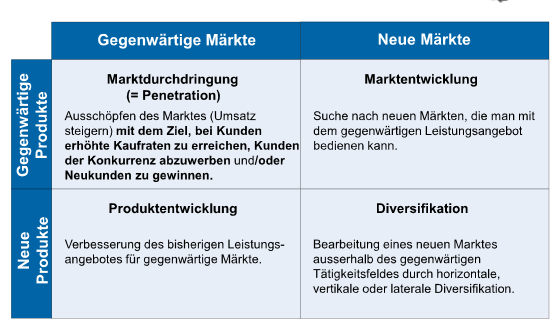
\includegraphics[width=0.3\textwidth]{Resources/Image/Ansoff.png}
\caption{\label{fig:Ansoff}Ansoff.}
\end{figure}
\pagebreak
\title\textbf{Die drei Stossrichtungen und ihre Erfolgsaussichten \\}

\begin{figure}[H]
\centering
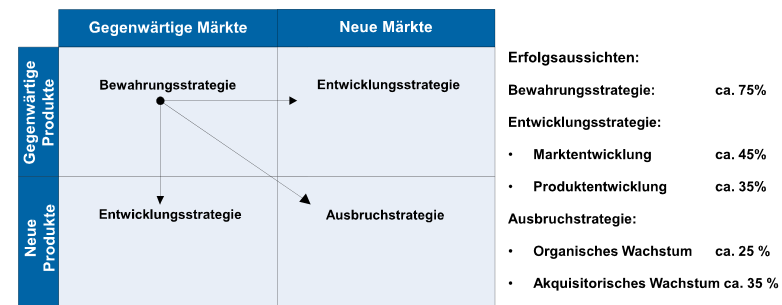
\includegraphics[width=0.3\textwidth]{Resources/Image/Stossrichtungen.png}
\caption{\label{fig:Stossrichtungen}Stossrichtungen.}
\end{figure}

\title\textbf{Marktdurchdringung\\}

\begin{figure}[H]
\centering
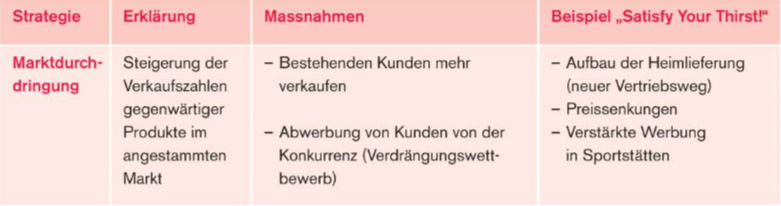
\includegraphics[width=0.3\textwidth]{Resources/Image/Marktdurchdringung.png}
\caption{\label{fig:Marktdurchdringung}Marktdurchdringung.}
\end{figure}


\title\textbf{Marktentwicklung\\}

\begin{figure}[H]
\centering
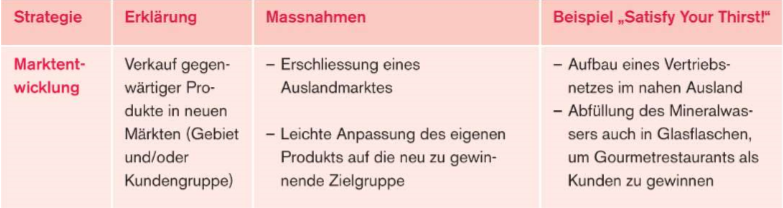
\includegraphics[width=0.3\textwidth]{Resources/Image/Marktentwicklung.png}
\caption{\label{fig:Marktentwicklung}Marktentwicklung.}
\end{figure}


\title\textbf{Produktentwicklung\\}

\begin{figure}[H]
\centering
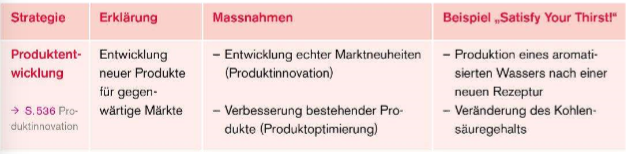
\includegraphics[width=0.3\textwidth]{Resources/Image/Produktentwicklung.png}
\caption{\label{fig:Produktentwicklung}Produktentwicklung.}
\end{figure}


\title\textbf{Diversifikation\\}
\begin{figure}[H]
\centering
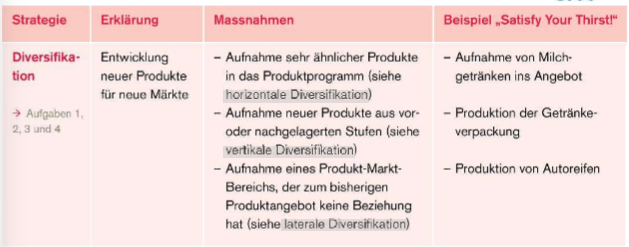
\includegraphics[width=0.3\textwidth]{Resources/Image/Diversifikation.png}
\caption{\label{fig:Diversifikation}Diversifikation.}
\end{figure}

\pagebreak
\section{Marketing I}


\textbf{Begriff: } Verstehen (Analyse) und Befriedigen (Aktivitäten, 4P-Mix) von Märkten und von Kundenbedürfnissen um die unternehmerische Ziele zu erreichen. \\

\begin{figure}[H]
\centering
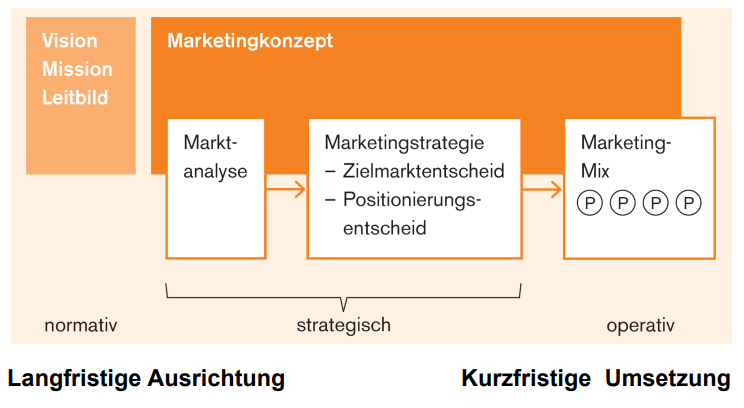
\includegraphics[width=0.3\textwidth]{Resources/Image/BegriffMarketing.png}
\caption{\label{fig:BegriffMarketing}BegriffMarketing.}
\end{figure}

\title{Absätzmärkte}

\begin{figure}[H]
\centering
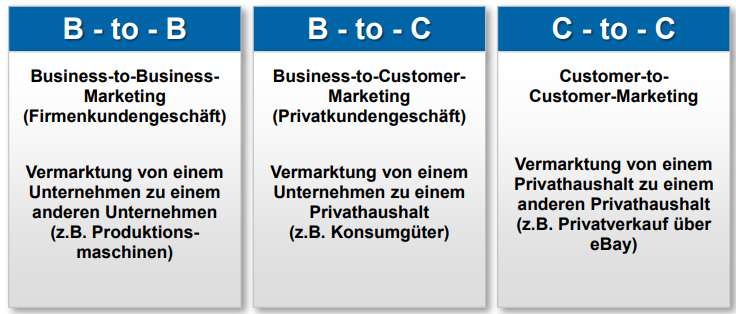
\includegraphics[width=0.3\textwidth]{Resources/Image/Absatzmarkt.png}
\caption{\label{fig:BegriffMarketing}BegriffMarketing.}
\end{figure}


\subsection{Marktanalyse}


														


\begin{tabular}{|l|l|l|}
\hline 
\textbf{Marktforschung} & \textbf{ Ziel} & {Typische Fragen} \\ 
\hline
\rule[-1ex]{0pt}{2.5ex}  
\textbf{Qualitativ} & Zahlenwerte über den Markt ermitteln & Marktvolumen?Marktanteil eines Unternehmens\\ 
\hline 
\textbf{Quantitativ} & Motive, Verhalten Kunden & Erwartungen, Warum kauft  \\ 
\hline 
\end{tabular} 

\subsubsection{Erhebungsmethoden}


\begin{multicols}{2}

\textbf{Field Research / Primärforschung}
\begin{itemize}
	\item Befragung Personen
	\item Gespräch Branchenexperten
	\item Besuch Veranstaltungen / Messen
	\item Stiller Beobachter
\end{itemize}

\columnbreak
\textbf{Desk Research/ Sekundärforschung}
\begin{itemize}
	\item Wissenschaftliche Publikationen
	\item Unternehmensinformationen
	\item Brancheniformation
	\item Öffentliche Informationen
	\item Sonstige Nachschlagewerke
\end{itemize}


\end{multicols}


\subsubsection{Marktgrössen}
\begin{figure}[H]
\centering
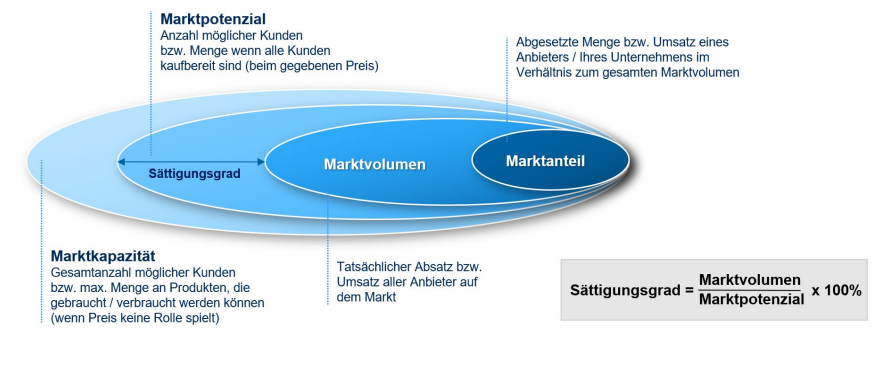
\includegraphics[width=0.3\textwidth]{Resources/Image/Marktgroessen.png}
\caption{\label{fig:BegriffMarketing}Marktgroessen .}
\end{figure}

\textbf{Marktsegmentierung}\\

\textbf{Definition: } Aufteilung des Gesamtmarktes in homogene Käufergruppen nach bestimmten Kriterien

\begin{multicols}{3}

\begin{figure}[H]
\centering
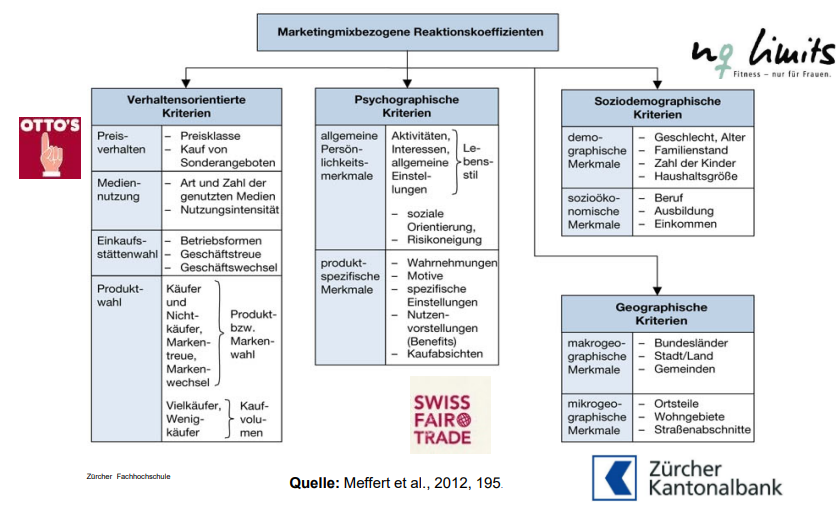
\includegraphics[width=0.3\textwidth]{Resources/Image/ModellSegmentierung.png}
\caption{\label{fig:ModellSegmentierung}ModellSegmentierung.}
\end{figure}


\columnbreak
\begin{figure}[H]
\centering
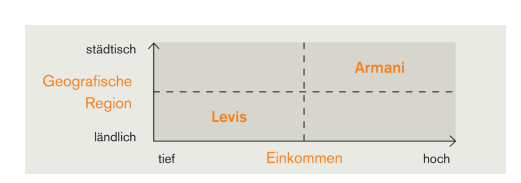
\includegraphics[width=0.3\textwidth]{Resources/Image/AbgrenzungGeographisch.png}
\caption{\label{fig:BegriffMarketing}AbgrenzungGeographisch.}
\end{figure}

\columnbreak
\begin{figure}[H]
\centering
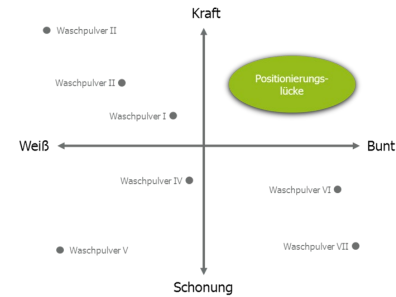
\includegraphics[width=0.3\textwidth]{Resources/Image/AbgrenzungEigenschaften.png}
\caption{\label{fig:AbgrenzungEigenschaften}AbgrenzungEigenschaften.}
\end{figure}



\end{multicols}

\subsection{Marketing 4P-Mix}


\begin{multicols*}{4}
\textcolor {orange} {\textbf{Product}}
\begin{itemize}
	\item Absatzprogramm / Sortiment
	\item Produkteigenschaften
	\item Verpackung
	\item Serviceleistungen
	\item Garantieleistungen
\end{itemize}


\columnbreak
\textcolor {orange} {\textbf{Price}}
\begin{itemize}
	\item Preisbestimmung
	\item Preisstrategie
	\item Konditionen
\end{itemize}

\columnbreak
\textcolor {orange} {\textbf{Place}}
\begin{itemize}
	\item Absatzwege
	\item Transportmittel
\end{itemize}

\columnbreak
\textcolor {orange} {\textbf{Promotion}}
\begin{itemize}
	\item Werbung
	\item Öffentlichkeitsarbeit
	\item Sponsoring
\end{itemize}


\end{multicols*}



\subsubsection{Produktgestaltung}

\begin{multicols*}{3}
\textcolor {orange} {\textbf{Gestaltung des Produktkerns (Grundnutzen)}}
\begin{itemize}
	\item Grösse
	\item Gewicht
	\item Material
	\item technische Leistung
	\item Bedienungsfreundlichkeit
\end{itemize}


\columnbreak
\textcolor {orange} {\textbf{Gestaltung des Produktäusseren(Zusatznutzen)}}
\begin{itemize}
	\item Design (Form, Farbe)
	\item Verpackung
	\item Markierung
\end{itemize}

\columnbreak
\textcolor {orange} {\textbf{Zusatzleisungen (Kundenservice)zum Produkt}}
\begin{itemize}
	\item Beratung
	\item Schulung
	\item Zustellung
	\item Installation
	\item Reparatur und Garantiedienst
\end{itemize}




\end{multicols*}


\title{Verpackung Funktionen}

\begin{multicols*}{2}
\textcolor {orange} {\textbf{Technische Funktionen}}
\begin{itemize}
	\item Transportfunktionen
	\item Lagerfunktionen
	\item Schutzfunktionen
\end{itemize}


\columnbreak
\textcolor {orange} {\textbf{Kommunikative Funktionen}}

\begin{itemize}
	\item Informationsfunktion
	\item Werbemittelfunktion
	
\end{itemize}

\end{multicols*}



\subsubsection{Preisstrategie}

\paragraph{Preishöhe: } Je höher der Preis, desto höher ist bei einer bestimmten Absatzmenge der Umsatz des Unternehmens.\\

\paragraph{Absatzmenge: } Der Preis beeinfluss die absetzbare Menge des Gutes. In der Regel sinkt die Absatzmenge eines Gutes bei steigendem Preis.

\title{3 Ansätze der Preisfestsetzung}

\begin{multicols*}{4}
\textcolor {orange} {\textbf{Nachfrageorientierung}}
\begin{itemize}
	\item Ausgangspunkt
	\begin{itemize}
		\item Zahlungsbereitschaft der Kunden
	\end{itemize}
\end{itemize}

\columnbreak

\textcolor {orange} {\textbf{Kostenorientierung}}
\begin{itemize}
	\item Ausgangspunkt
	\begin{itemize}
		\item Kosten des Produkts für das Unternehmen
	\end{itemize}
\end{itemize}

\columnbreak

\textcolor {orange} {\textbf{Wettbewerbsorientierung}}
\begin{itemize}
	\item Ausgangspunkt
	\begin{itemize}
		\item Preise der Konkurrenz
	\end{itemize}
\end{itemize}
	
\columnbreak
\begin{figure}[H]
\centering
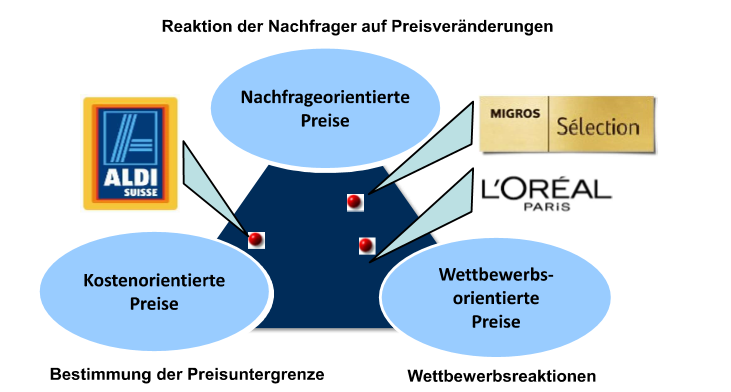
\includegraphics[width=0.3\textwidth]{Resources/Image/ReaktionNachfrager.png}
\caption{\label{fig:ReaktionNachfrager}ReaktionNachfrager.}
\end{figure}

\end{multicols*}


\title{Die Break-Even-Analyse}

\paragraph{Defintion: } Bewertungsmodell zur Ermittlung der Absatzmenge, die erforderlich ist, um die Gewinnschwelle zu erreichen.

\begin{figure}[H]
\centering
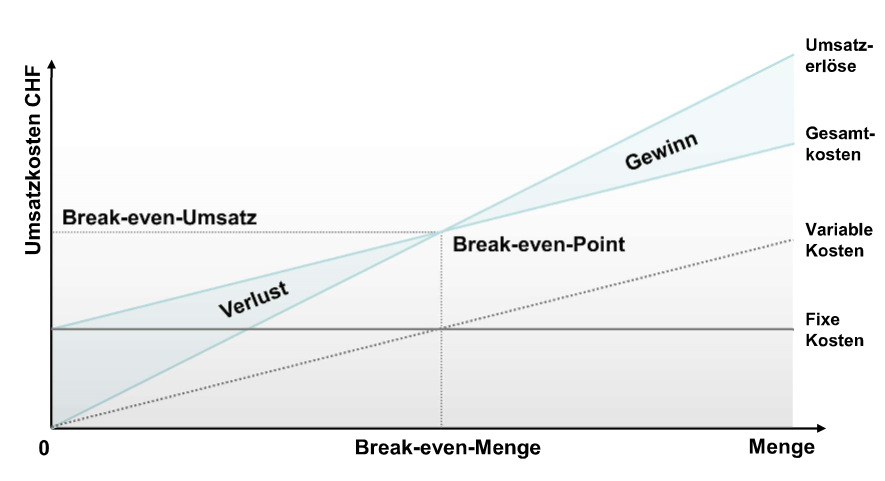
\includegraphics[width=0.3\textwidth]{Resources/Image/Break-Even-Analyse.png}
\caption{\label{fig:BreakEvenAnalyse}BreakEvenAnalyse.}
\end{figure}






































































































































































































































\end{document}